%%%%%%%%%%%%%%%%%%%%%%%%%%%%%%%%%%%%%%%%%%%%%%%%%%%%%%%%%%%%%%%%%%%%%%%%%%%%%%%%%%
\begin{frame}[fragile]\frametitle{}
\begin{center}
{\Large Introduction}
\end{center}
\end{frame}


%%%%%%%%%%%%%%%%%%%%%%%%%%%%%%%%%%%%%%%%%%%%%%%%%%%%%%%%%%%%%%%%%%%%%%%%%%%%%%%%%%
\begin{frame}[fragile]\frametitle{Introduction to Yoganidra}
	\begin{itemize}
		\item \textbf{Yoga Nidra (योगनिद्रा)} is a deep relaxation technique that:
			\begin{itemize}
				\item Relieves stress.
				\item Improves sleep.
				\item Accesses the bliss state (Ananda आनन्द).
			\end{itemize}
	\item Composed of series of body, breath, imagination acts to guide into progressive states of relaxation (non-doing)
    \item \textbf{Inspired by the Bihar School of Yoga}, this script follows the inward journey through the Koshas.
	\end{itemize}
	
\end{frame}

%%%%%%%%%%%%%%%%%%%%%%%%%%%%%%%%%%%%%%%%%%%%%%%%%%%%%%%%%%%
\begin{frame}[fragile]\frametitle{What is Yoga Nidra?}
      \begin{center}
        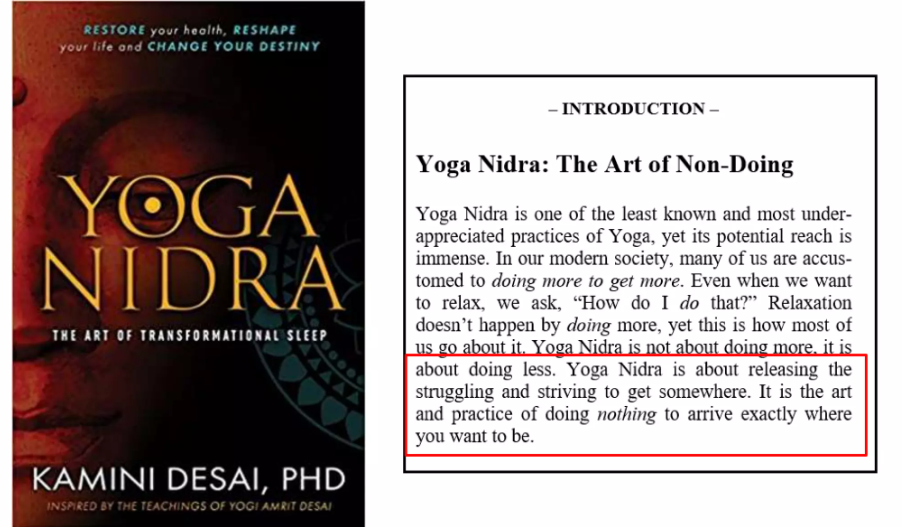
\includegraphics[width=\linewidth,keepaspectratio]{yoganidra1}

		{\tiny (Ref: Yoga Nidra - Dr Amit Chail)}		
        \end{center}

\end{frame}

%%%%%%%%%%%%%%%%%%%%%%%%%%%%%%%%%%%%%%%%%%%%%%%%%%%%%%%%%%%
\begin{frame}[fragile]\frametitle{What is Yoga Nidra?}
Its is Pratyahara प्रत्याहार  : Prati प्रति (inside) + ahara आहार  (food), ie food to inside, that is, contrary to our attention being always external looking, here we are looking inside. Plus, there is tantra word 'nyasa' न्यास , meanings seating. meaning you put attention at different places.

      \begin{center}
        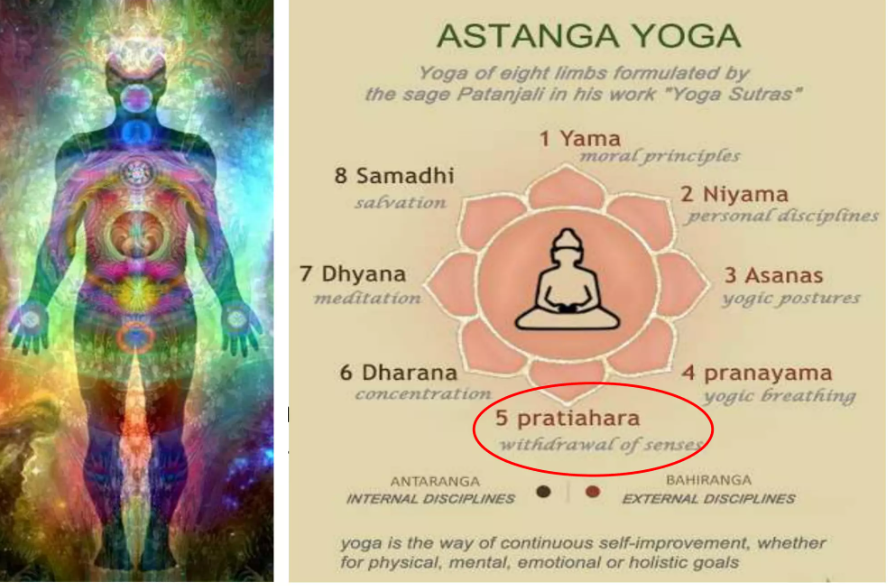
\includegraphics[width=0.6\linewidth,keepaspectratio]{yoganidra2}

		{\tiny (Ref: Yoga Nidra - Dr Amit Chail)}		
        \end{center}

\end{frame}

%%%%%%%%%%%%%%%%%%%%%%%%%%%%%%%%%%%%%%%%%%%%%%%%%%%%%%%%%%%
\begin{frame}[fragile]\frametitle{History}
      \begin{center}
        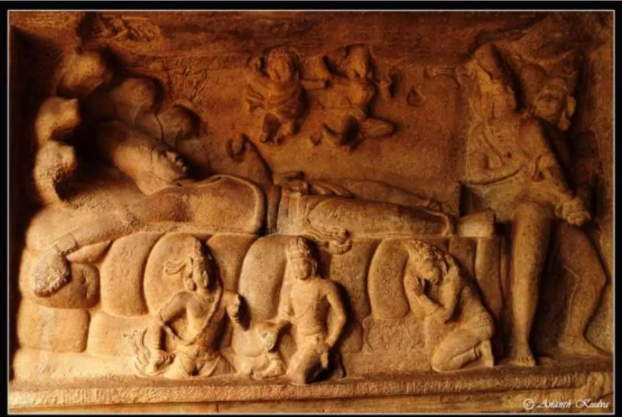
\includegraphics[width=0.8\linewidth,keepaspectratio]{yoganidra3}

		{\tiny (Ref: Yoga Nidra - Dr Amit Chail)}		
        \end{center}

\end{frame}

%%%%%%%%%%%%%%%%%%%%%%%%%%%%%%%%%%%%%%%%%%%%%%%%%%%%%%%%%%%
\begin{frame}[fragile]\frametitle{Four Stages of Human Consciousness}
      \begin{center}
        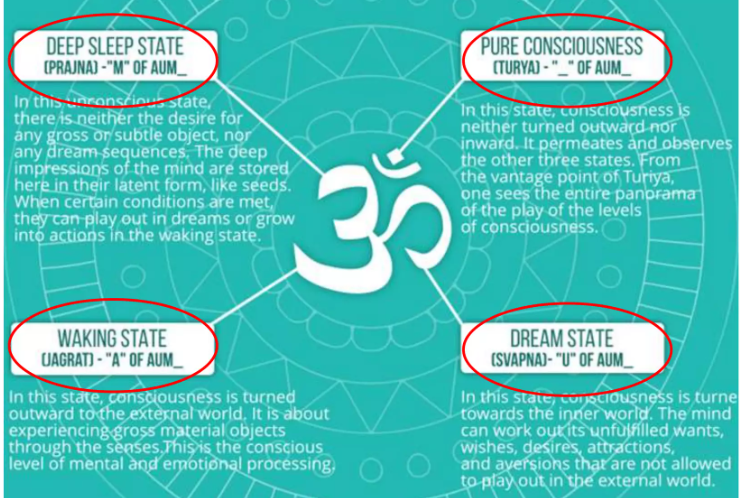
\includegraphics[width=0.8\linewidth,keepaspectratio]{yoganidra4}

		{\tiny (Ref: Yoga Nidra - Dr Amit Chail)}		
        \end{center}

\end{frame}

%%%%%%%%%%%%%%%%%%%%%%%%%%%%%%%%%%%%%%%%%%%%%%%%%%%%%%%%%%%
\begin{frame}[fragile]\frametitle{Practitioners}
      \begin{center}
        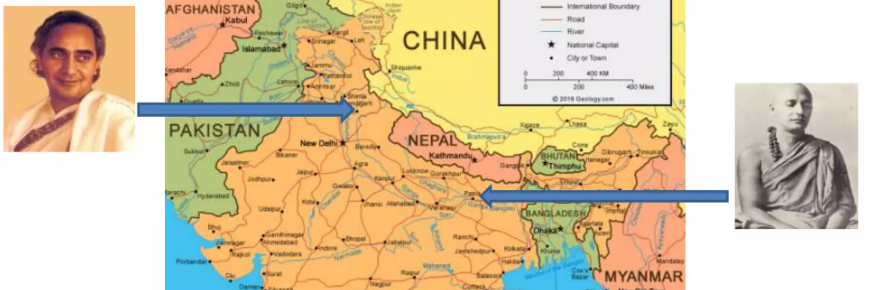
\includegraphics[width=\linewidth,keepaspectratio]{yoganidra5}

		{\tiny (Ref: Yoga Nidra - Dr Amit Chail)}		
        \end{center}

\end{frame}

%%%%%%%%%%%%%%%%%%%%%%%%%%%%%%%%%%%%%%%%%%%%%%%%%%%%%%%%%%%
\begin{frame}[fragile]\frametitle{Modern Development}
    \textbf{Swami Satyananda Saraswati's Contributions:}
    \begin{itemize}
        \item Systematized Yoga Nidra in the 20th century
        \item Founded Bihar School of Yoga
        \item Made the practice accessible to modern practitioners
        \item Emphasized scientific approach to traditional practice
        \item Developed structured methodology for teaching
    \end{itemize}
\end{frame}

%%%%%%%%%%%%%%%%%%%%%%%%%%%%%%%%%%%%%%%%%%%%%%%%%%%%%%%%%%%
\begin{frame}[fragile]\frametitle{Research}
      \begin{center}
        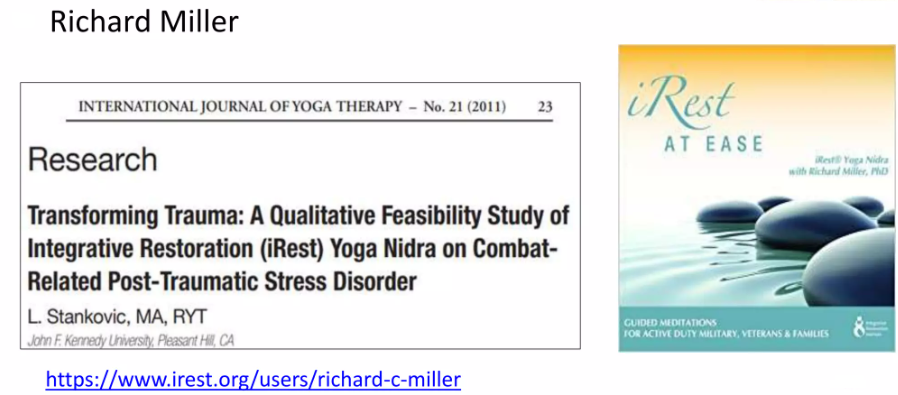
\includegraphics[width=\linewidth,keepaspectratio]{yoganidra6}

		{\tiny (Ref: Yoga Nidra - Dr Amit Chail)}		
        \end{center}

\end{frame}


%%%%%%%%%%%%%%%%%%%%%%%%%%%%%%%%%%%%%%%%%%%%%%%%%%%%%%%%%%%%%%%%%%%%%%%%%%%%%%%%%%
\begin{frame}[fragile]\frametitle{Nidra vs Yoganidra}
    \textbf{Nidra (निद्रा)}: \\
    \begin{itemize}
        \item Unaware, only physical relaxation.
        \item Unconscious state.
    \end{itemize}
    \vspace{5mm}
    \textbf{Yoganidra (योगनिद्रा)}: \\
    \begin{itemize}
        \item Aware relaxation (physical, mental, and emotional).
        \item Conscious of subconscious mind.
    \end{itemize}
\end{frame}

%%%%%%%%%%%%%%%%%%%%%%%%%%%%%%%%%%%%%%%%%%%%%%%%%%%%%%%%%%%%%%%%%%%%%%%%%%%%%%%%%%
\begin{frame}[fragile]\frametitle{Meditation vs Yoganidra}
    \begin{columns}
        \begin{column}{0.48\textwidth}
            \textbf{Meditation:}
            \begin{itemize}
                \item Typically done sitting up
                \item Focuses on one point of concentration
                \item Requires active mental effort
                \item May be challenging for beginners
            \end{itemize}
        \end{column}
        \begin{column}{0.48\textwidth}
            \textbf{Yoga Nidra:}
            \begin{itemize}
                \item Done lying down
                \item Systematic rotation of awareness
                \item Guided relaxation practice
                \item Accessible to all skill levels
            \end{itemize}
        \end{column}
    \end{columns}
\end{frame}

%%%%%%%%%%%%%%%%%%%%%%%%%%%%%%%%%%%%%%%%%%%%%%%%%%%%%%%%%%%
\begin{frame}[fragile]\frametitle{Science: ECG}
      \begin{center}
        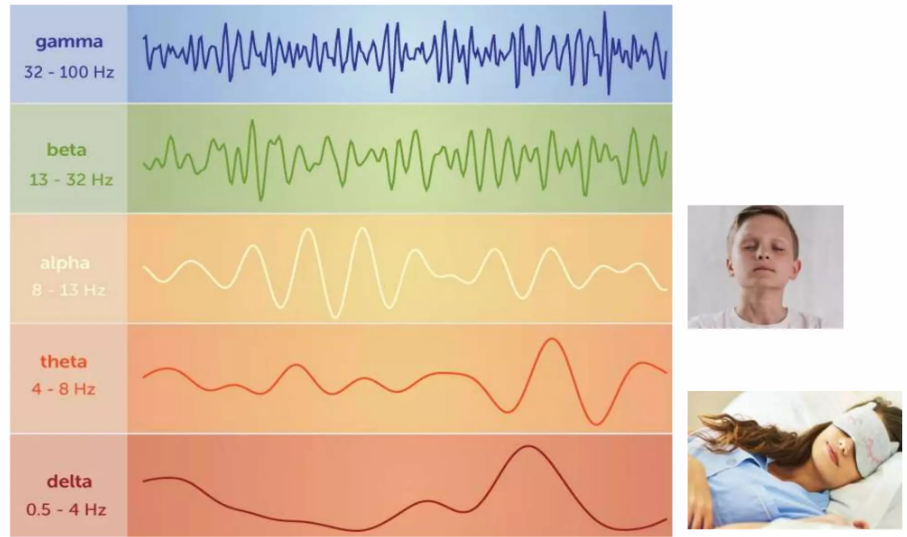
\includegraphics[width=\linewidth,keepaspectratio]{yoganidra9}

		{\tiny (Ref: Yoga Nidra - Dr Amit Chail)}		
        \end{center}

\end{frame}

%%%%%%%%%%%%%%%%%%%%%%%%%%%%%%%%%%%%%%%%%%%%%%%%%%%%%%%%%%%
\begin{frame}[fragile]\frametitle{Science: ECG}
      \begin{center}
        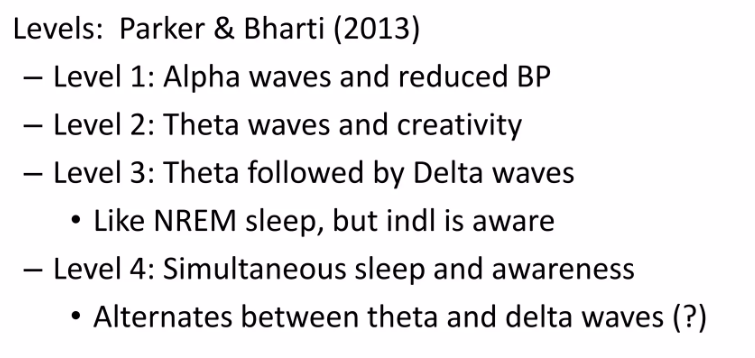
\includegraphics[width=0.8\linewidth,keepaspectratio]{yoganidra10}

		{\tiny (Ref: Yoga Nidra - Dr Amit Chail)}		
        \end{center}

\end{frame}



%%%%%%%%%%%%%%%%%%%%%%%%%%%%%%%%%%%%%%%%%%%%%%%%%%%%%%%%%%%%%%%%%%%%%%%%%%%%%%%%%%
\begin{frame}[fragile]\frametitle{8 Stages of Yoganidra}
    \begin{enumerate}
        \item \textbf{Preparation (Shavasana)}: Deep breaths in Shavasana (शवासन).
        \item \textbf{Resolve (Sankalpa)}: Optional positive affirmation (संकल्प).
        \item \textbf{Body Awareness (Rotation)}: Relax body parts.
        \item \textbf{Breath Awareness}: Relaxation through breath.
        \item \textbf{Opposite Sensations}: Experience and release emotions.
        \item \textbf{Visualization}: Reach the subconscious with imagery.
        \item \textbf{Resolve (Sankalpa)}: Repeat the Sankalpa again.
        \item \textbf{Exiting}: Return awareness to external surroundings.
    \end{enumerate}
\end{frame}

%%%%%%%%%%%%%%%%%%%%%%%%%%%%%%%%%%%%%%%%%%%%%%%%%%%%%%%%%%%%%%%%%%%%%%%%%%%%%%%%%%
\begin{frame}[fragile]\frametitle{Key Instructions}
    \begin{itemize}
        \item No movement during Yoganidra.
        \item Stay awake, do not fall asleep.
        \item Do not think, just follow the instructions.
    \end{itemize}
\end{frame}


%%%%%%%%%%%%%%%%%%%%%%%%%%%%%%%%%%%%%%%%%%%%%%%%%%%%%%%%%%%%%%%%%%%%%%%%%%%%%%%%%%
\begin{frame}[fragile]\frametitle{The Koshas (कोश)}
    \begin{itemize}
        \item \textbf{Annamaya Kosha (अन्नमयकोश)} - Physical Body
        \item \textbf{Pranamaya Kosha (प्राणमयकोश)} - Energy Body
        \item \textbf{Manomaya Kosha (मनोमयकोश)} - Emotional Body
        \item \textbf{Vijnanamaya Kosha (विज्ञानमयकोश)} - Wisdom Body
        \item \textbf{Anandamaya Kosha (आनन्दमयकोश)} - Bliss Body
    \end{itemize}
\end{frame}

%%%%%%%%%%%%%%%%%%%%%%%%%%%%%%%%%%%%%%%%%%%%%%%%%%%%%%%%%%%%%%%%%%%%%%%%%%%%%%%%%%
\begin{frame}[fragile]\frametitle{Koshas in Yoganidra}
    
    \begin{itemize}
        \item Body Awareness (Rotation): \textbf{Annamayakosha (अन्नमयकोश) - Physical Body:} Focus on different body parts (right palm, right arm, legs, back, etc.).
        \item Breath Awareness: \textbf{Pranamayakosha (प्राणमयकोश) - Breath Awareness:} Reverse breath count from 27.
        \item Opposite Sensations: \textbf{Manomayakosha (मनोमयकोश) - Emotional Body:} Experience opposite sensations (hot/cold, wet/dry).
        \item Visualization: \textbf{Vijnanamayakosha (विज्ञानमयकोश) - Subconscious Visualization:} Visualize calming scenes like deserts, lakes, and waves.
    \end{itemize}
\end{frame}

%%%%%%%%%%%%%%%%%%%%%%%%%%%%%%%%%%%%%%%%%%%%%%%%%%%%%%%%%%%%%%%%%%%%%%%%%%%%%%%%%%
\begin{frame}[fragile]\frametitle{Tips for Practicing Yoganidra}
    \begin{itemize}
        \item Use simple and precise language in the script.
        \item Speak in a clear and even tone.
        \item Sit comfortably and be still during facilitation.
        \item Practice in a warm, comfortable space. Use props (pillows, blankets) to support the body.
        \item Remain still, but do not fall asleep.
    \end{itemize}
\end{frame}

%%%%%%%%%%%%%%%%%%%%%%%%%%%%%%%%%%%%%%%%%%%%%%%%%%%%%%%%%%%
\begin{frame}[fragile]\frametitle{Important Considerations}
    \begin{itemize}
        \item \textbf{Consult Healthcare Provider if:}
        \begin{itemize}
            \item Pregnant or recently post-partum
            \item Have serious medical conditions
            \item Experiencing severe mental health issues
        \end{itemize}
        \item \textbf{Practice Guidelines:}
        \begin{itemize}
            \item Avoid practice immediately after meals
            \item Ensure comfortable room temperature
            \item Practice at consistent times
            \item Stay awake during the practice
        \end{itemize}
    \end{itemize}
\end{frame}